\section{Inledning}
Denna rapport redovisar de test som utförts och skapats under iteration 2 i projektet. I första delen beskrivs hur testproceduren gått till samt vilka som delatagit. Sedan efter det beskrivs de objekt som har testats.
\subsection{Deltagare}
Genom hela iteration 2 har samtliga gruppmedlemmar jobbat med testning. Johan, Alexander och Ruben har fortsatt testandet av lösaren, Martin har fortsatt testa ny kod i matrisbiblioteket, Adam har testat ny funktionalitet i parsern, och Dennis och Sebastian har jobbat med integrationen mot matlab där test av matrisomvandligar har krävts. 

\subsection{Procedur}
Under iteration 2 har fler delar integrerats med varandra, till exempel som att lösaren har kopplats ihop med matlab. Detta har lett till att projektmedlemmarna jobbat mer tillsammans och på ett effektivare sätt kunnat testa koden. Testen har fortfarande bestått utav Black-Box-test, men denna gång varit mer övergripande. Här är ett exempel på ett test utav lösaren:

$$quadopt\_solver(problem);$$
$$assert(compare\_matrices(problem\rightarrow solution, expected\_ans));$$

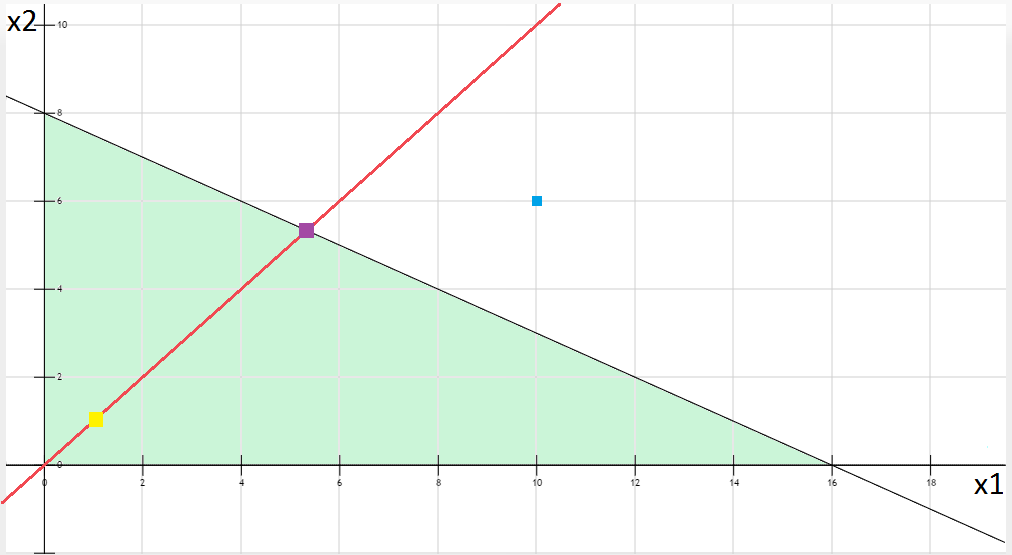
\includegraphics[scale=0.6]{prob.png}


\raggedright I bilden ovan är det gröna området det tillåtna rummet som spänns upp utav ''$\geq$''-bivillkoren. Det röda sträcket är ett ''$=$''-bivillkor (alltså ett bivillkor där punkten måste ligga på linjen). Den blåa pricken är målfunktionens globala minimum, den gula pricken är startpunkten och den lila är optimum. \newline
Om problem i testet är som beskrivet i bilden ovan, så skulle variabeln ''problem'' beskriva hela problemet, och ''expected\_ans'' vara den förväntade optimala punkten (lila pricken). Om asserten misslyckas betyder det att lösaren inte lyckades lösa problemet.

